\chapter{RESULTS AND DISCUSSIONS}
\thispagestyle{empty}
\onehalfspacing
\pagestyle{fancy}
\fancyhf{}
\fancyhead[LE,RO]{\textit{\footnotesize \thepage}}
\fancyhead[RE,LO]{\textit{\footnotesize Application of IoT in Agriculture}}
%\fancyfoot[LE,LO]{\textit{\footnotesize Department of CSE}}
\fancyfoot[LE,RO]{\textit{\footnotesize Department of CSE}}
 
\renewcommand{\headrulewidth}{2pt}
\renewcommand{\footrulewidth}{1pt}
\section{Calculation of Confusion Matrix}\\
\par In classification issues, classification models are used to forecast the target class data sample. The likelihood that each occurrence belongs to one class or another is predicted by the categorization model. The confusion matrix is a matrix representation of TP, TN, FP, and FN. These are the three models' confusion matrices.\\\\
\par TP is 380, FP is 46, FN is 4, and TN is 461 in the CNN confusion matrix. In this case, the plastic is forecasted to be 461 and the non-plastic is 380 as expected.
\begin{figure}
    \centering
    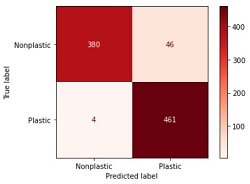
\includegraphics{cnn-cm1.jpg}
    \caption{Confusion Matrix of CNN}
    \label{Confusion Matrix of CNN}
\end{figure}
\par In the Random Forest confusion matrix, the TP is 403, FP is 23, FN is 0, and TN is 465. In this instance, it is anticipated that the plastic will be 465 and the non-plastic will be 403.
\begin{figure}
    \centering
    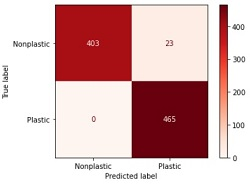
\includegraphics{rf-cm1.jpg}
    \caption{Confusion Matrix of Random Forest}
    \label{Confusion Matrix of Random Forest}
\end{figure}
\begin{figure}
    \centering
    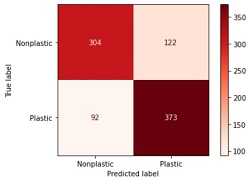
\includegraphics{ngb-cm1.jpg}
    \caption{Confusion Matrix of Gaussian Naive Bayes}
    \label{Confusion Matrix of Gaussian Naive Bayes}
\end{figure}
\newpage   
\subsection{Calculation of Parameters}
To study the three models, calculate the values of the following parameters.\\
\text{1. Accuracy}
\par The proportion of true positives and true negatives to all positive and negative observations is used to calculate the accuracy of a machine learning model. In other words, accuracy measures how often we can assume that our machine will correctly forecast the outcome based on all of the predicted iterations. The accuracy score derived from the confusion matrix above is displayed in the table below.\\
\begin{center}
    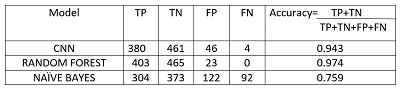
\includegraphics[]{tb1.jpg}
\end{center}
\par From the calculations, Random Forests achieved the highest accuracy score, i.e.
97\%. The accuracy score is then plotted as follows
\begin{center}
    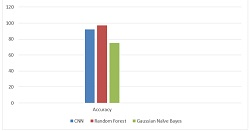
\includegraphics[]{acc2.jpg}
\end{center}
\text{2. Precision}
\par The percentage of positively predicted labels that are really correct is represented by the model's accuracy score. Positive predictive value and precision are both synonyms. False positives and false negatives are balanced using precision and recall. Class distribution affects precision. The following table represents the precision score from the above mentioned confusion matrix:
\begin{center}
    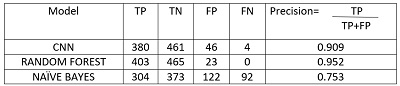
\includegraphics[]{tb2.jpg}
\end{center}
\par After calculation, the precision score of Random Forests is higher than CNN \& Gaussian Naive Bayes. The precision score is then plotted as follows
\begin{center}
    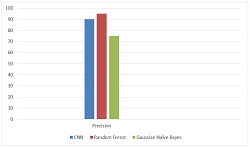
\includegraphics[]{g1.jpg}
\end{center}
\text{3. Recall}
\par The model's recall score shows how well it can distinguish false positives from real positives. This is in contrast to precision, which assesses the proportion of a model's positive predictions that come to pass. The following table represents the recall score from the confusion matrix mentioned above:
\begin{center}
    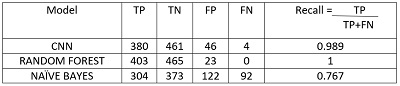
\includegraphics[]{tb3.jpg}
\end{center}
\par The table shows that Random Forest achieved the highest recall score. The recall score is then plotted as follows
\begin{center}
    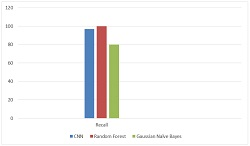
\includegraphics[]{g2.jpg}
\end{center}
\text{4. F1- Score}
\par The precision and recall scores are functions of the model score, which is represented by the F1 model score. F-score is a substitute for the accuracy metrics in the following table since it measures the accuracy performance of machine learning models by equally weighting precision and recall:
\begin{center}
    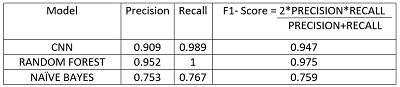
\includegraphics[]{tb4.jpg}
\end{center}
\par The highest F1 score belongs to Random Forest. Next, the F1 score is plotted as shown.
\begin{center}
    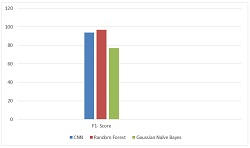
\includegraphics[]{g3.jpg}
\end{center}

\text{5. ROC}
\par It also got simple to compare various three predictors on a certain data set. The area under the curve, or ROC, is all that matters; the greater the number, the better. The appropriate threshold for differentiating positive and negative samples is determined using ROC curves, which are used to assess how successfully your classifier can do so. ROC curves summarise the trade-off between the true positive rate and false positive rate for a predictive model using different probability thresholds. It is possible to choose the ideal operating point using the ROC curve. The three models' ROCs are as follows.
\begin{center}
    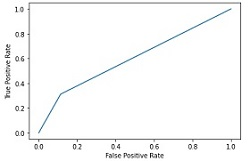
\includegraphics[]{rc1.jpg}\\
    \text{ROC of CNN}
\end{center}
\begin{center}
     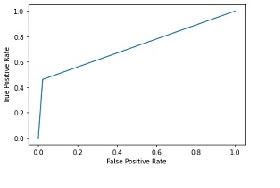
\includegraphics[]{rc2.jpg}\\
    \text{ROC of Random Forest}
\end{center}
\begin{center}
    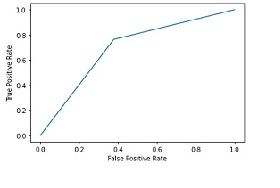
\includegraphics[]{rc3.jpg}\\
    \text{ROC of Gaussian Naive Bayes}
\end{center}
















